\documentclass[10pt]{report}
\usepackage{./EE703handout}
\usepackage{tikz}
\usepackage{pgfplots}
\usetikzlibrary{decorations.pathmorphing}
\usepackage{mathtools}
\usepackage{subfig}
\usepackage{hyperref}
\usepackage{enumitem}
\usepackage{verbatim}
\usetikzlibrary{arrows,backgrounds,shapes,matrix,positioning,fit}
\setlength{\textheight}{9.4in}     % 9.4in
\setlength{\textwidth}{7.3in}      % 6.3in
\setlength{\parindent}{0mm}
%\setlength{\parskip}{3mm}
\setlength{\oddsidemargin}{-0.5in}  % 0.0in
\setlength{\topmargin}{-1.0in}  % 0.0in
\setlength{\headheight}{0.0in}  % 0.0in

\renewcommand\Re{\operatorname{Re}}

\begin{document}
\handout{}{Date: September 10, 2013}{Midsem Exam: \textbf{30 points}}
Each question is worth 5 points.
\begin{enumerate}
  \item Let $u_p(t)$ and $v_p(t)$ be passband signals centered at the same carrier frequency $f_c$. Let $u(t) = u_c(t)+ju_s(t)$ and $v(t) = v_c(t) + jv_s(t)$ be the complex baseband representations of $u_p(t)$ and $v_p(t)$ respectively. Prove that
  \begin{equation*}
    \langle u_p,v_p \rangle = \langle u_c,v_c \rangle + \langle u_s,v_s \rangle = \Re\left(\langle u,v \rangle\right).
  \end{equation*}
  \item Suppose the Gram-Schmidt orthogonalization procedure is performed on a set of $M$ signals $s_1(t), \ldots, s_M(t)$ to obtain an orthonormal basis $\phi_1(t), \ldots, \phi_N(t)$.
  \begin{enumerate}
    \item In which situation is $N$ equal to one? Give a condition on the signals $s_i(t), 1 \leq i \leq M$.
    \item In which situation is $N$ equal to $M$? Give a condition on the signals $s_i(t), 1 \leq i \leq M$.
    \item In which situation is $N$ equal to $M-1$? Give a condition on the signals $s_i(t), 1 \leq i \leq M$.
    \item If $\sum_{i=1}^M s_i(t) = 0$ for all $t$, what can you say about the orthonormal basis $\phi_1(t), \ldots, \phi_N(t)$?
    \item Can $\sum_{i=1}^N \phi_i(t)$ be equal to zero for all $t$? Explain why or why not.
  \end{enumerate}
  \item Determine the power spectral density of the following line coding scheme:
    \begin{equation*}
      u(t) = \sum_{n=-\infty}^{\infty} b_n p(t-nT)
    \end{equation*}
    where $p(t) = I_{[0,T)}(t)$ and the symbol $b_n$ is the obtained by mapping a zero bit to amplitude $-A$ and mapping a one bit to amplitude $2A$. Assume that the bits used to generate $b_n$ are independent and equally likely to be zero or one. Simplify your answer such that it does not contain any infinite summations. The formula for the PSD is as follows.
    \begin{equation*}
      S_u(f) = \frac{\lvert P(f)\rvert^2}{T}\sum_{k=-\infty}^{\infty} R_b[k] e^{\ -j2\pi kfT}
    \end{equation*}
  \item The constellation $s_0 = -3A, s_1 = -A, s_2 = 0, s_3 = 2A$ is corrupted by noise $N$ which is a zero mean Gaussian random variable having variance $\sigma^2$. Assume all four constellation points are equally likely to be transmitted. 
    \begin{enumerate}
      \item Find the optimal decision rule based on the observation Y.
      \item Find the average probability of decision error for the optimal decision rule. Express your final answer in terms of the $Q$ function.
    \end{enumerate}
    \begin{figure}[h]
      \centering
        \begin{tikzpicture}[scale=1.0,transform shape]
          \node at (0,0) (si) {$s_i$};
          \node[circle, draw, right=1 of si] (plus) {$+$};
          \node[above=1 of plus] (noise) {$N$};
          \node[right=1 of plus] (y) {$Y$};
          \draw[->,very thick] (noise) -- (plus);
          \draw[->,very thick] (plus) -- (y);
          \draw[->,very thick] (si) -- (plus);
        \end{tikzpicture}
      \centering
        \begin{tikzpicture}[scale=0.75,transform shape]
          \begin{axis}[
                       xmax=3.5,
                       xmin=-3.5,
                       ymax=0.1,
                       ymin=-0.1,
                       axis lines = middle,
                       ytick=\empty,
                       xtick = data,
                       x post scale = 2.0,
                       xticklabel shift = -20pt,
                       xticklabels = {$-3A$,$-A$,0,$2A$},
                       x post scale = 2.0,
                      ]
            \addplot+[only marks, mark options={draw=black,fill=black},] coordinates {(-3,0) (-1,0) (0.01,0) (2,0)};
          \end{axis}
        \end{tikzpicture}
    \end{figure}

  \item Suppose an encoder maps a 0 bit to a binary codeword $\mathbf{v}_0$ of length $n$ and maps a 1 bit to a binary codeword $\mathbf{v}_1$ of length $n$. The codewords are passed through a binary symmetric channel with crossover probability $p$. Suppose $\mathbf{r}$ is the received word corresponding to a single transmitted codeword. If $\mathbf{v}_0$ and $\mathbf{v}_1$ share the same prefix\footnote{For instance, codewords 01011 and 01001 share a prefix of length 3} of length $k < n$, show that the optimal decoder can ignore the first $k$ bits in the received word $\mathbf{r}$. Assume that the probability of a 0 bit appearing at the input to the encoder is $\pi_0$ and the probability of a 1 bit appearing at the input to the encoder is $\pi_1$.

  \item Suppose the input to the following binary channel is equally likely to be 0 or 1. Assuming $0 \leq p < \frac{1}{2}$, derive the minimum probability of decision error which can be achieved for this channel as a function of $p$.

  \begin{figure}[h]
    \centering
      \begin{tikzpicture}[scale=1.2,transform shape]
        \node (zeroinput) {0};
        \node[below = 2cm of zeroinput] (oneinput) {1};
        \node[right = 4cm of zeroinput] (zerooutput) {0};
        \node[below = 2cm of zerooutput] (oneoutput) {1};
        \draw [->,very thick] (zeroinput) to node[above] {$1-2p$} (zerooutput);
        \draw [->,very thick] (oneinput) to node[below] {$1-p$}  (oneoutput);
        \draw [->,very thick] (zeroinput) to  (oneoutput);
        \draw [->,very thick] (oneinput) to  (zerooutput);
        \node[above right = 0.65cm of oneinput] {$p$};
        \node[below right = 0.65cm of zeroinput] {$2p$};
      \end{tikzpicture}
  \end{figure}

\end{enumerate}
\end{document}
